\documentclass[a4paper,11pt]{article}
\usepackage{amsmath,amsthm,amsfonts,amssymb,amscd,amstext,vmargin,graphics,graphicx,tabularx,multicol} 
\usepackage[francais]{babel}
\usepackage[utf8]{inputenc}  
\usepackage[T1]{fontenc} 
\usepackage{pstricks-add,tikz,tkz-tab,variations}
\usepackage[autolanguage,np]{numprint} 

\setmarginsrb{1.5cm}{0.5cm}{1cm}{0.5cm}{0cm}{0cm}{0cm}{0cm} %Gauche, haut, droite, haut
\newcounter{numexo}
\newcommand{\exo}[1]{\stepcounter{numexo}\noindent{\bf \underline{Exercice~\thenumexo}}}
\reversemarginpar


\newcounter{enumtabi}
\newcounter{enumtaba}
\newcommand{\q}{\stepcounter{enumtabi} \theenumtabi.  }
\newcommand{\qa}{\stepcounter{enumtaba} (\alph{enumtaba}) }
\newcommand{\initq}{\setcounter{enumtabi}{0}}
\newcommand{\initqa}{\setcounter{enumtaba}{0}}

\newcommand{\be}{\begin{enumerate}}
\newcommand{\ee}{\end{enumerate}}
\newcommand{\bi}{\begin{itemize}}
\newcommand{\ei}{\end{itemize}}
\newcommand{\bp}{\begin{pspicture*}}
\newcommand{\ep}{\end{pspicture*}}
\newcommand{\bt}{\begin{tabular}}
\newcommand{\et}{\end{tabular}}
\renewcommand{\tabularxcolumn}[1]{>{\centering}m{#1}} %(colonne m{} centrée, au lieu de p par défault) 
\newcommand{\tnl}{\tabularnewline}

\newcommand{\bmul}[1]{\begin{multicols}{#1}}
\newcommand{\emul}{\end{multicols}}

\newcommand{\trait}{\noindent \rule{\linewidth}{0.2mm}}
\newcommand{\hs}[1]{\hspace{#1}}
\newcommand{\vs}[1]{\vspace{#1}}

\newcommand{\N}{\mathbb{N}}
\newcommand{\Z}{\mathbb{Z}}
\newcommand{\R}{\mathbb{R}}
\newcommand{\C}{\mathbb{C}}
\newcommand{\Dcal}{\mathcal{D}}
\newcommand{\Ccal}{\mathcal{C}}
\newcommand{\mc}{\mathcal}

\newcommand{\vect}[1]{\overrightarrow{#1}}
\newcommand{\ds}{\displaystyle}
\newcommand{\eq}{\quad \Leftrightarrow \quad}
\newcommand{\vecti}{\vec{\imath}}
\newcommand{\vectj}{\vec{\jmath}}
\newcommand{\Oij}{(O;\vec{\imath}, \vec{\jmath})}
\newcommand{\OIJ}{(O;I,J)}




\newcommand{\reponse}[1][1]{%
\multido{}{#1}{\makebox[\linewidth]{\rule[0pt]{0pt}{20pt}\dotfill}
}}

\newcommand{\titre}[5] 
% #1: titre #2: haut gauche #3: bas gauche #4: haut droite #5: bas droite
{
\noindent #2 \hfill #4 \\
#3 \hfill #5

\vspace{-1.6cm}

\begin{center}\rule{6cm}{0.5mm}\end{center}
\vspace{0.2cm}
\begin{center}{\large{\textbf{#1}}}\end{center}
\begin{center}\rule{6cm}{0.5mm}\end{center}
}



\begin{document}
\pagestyle{empty}
\titre{Chapitre 13 : Organisation et représentation de données}{}{}{}{}

\vspace*{1cm}
Exercices 7/8/9 p 109

Exercices 5 p 60 8 p 57
\renewcommand{\arraystretch}{2.5}


\begin{center}
{\Large \textbf{Niveau 1 :}}
\end{center}

\vspace*{1cm}

$\rightarrow$ \textbf{Exploiter un diagramme}\\

\vspace*{0.5cm}


\exo \\ Le tableau d'élèves ci-dessous indique la répartition des papillons dans les terrariums de Vincent, Fiona et Florence.\\

	\begin{tabular}{|c|c|c|c|}
	\hline 
	 & Vincent & Fiona & Florence \\ 
	\hline 
	Papillons rouges & 1 & 1 & 2 \\ 
	\hline 
	Papillons bleus & 1 & 2 & 2 \\ 
	\hline 
	Papillons verts & 6 & 1 & 2 \\ 
	\hline 
	\end{tabular} 
	
	\vspace*{1cm}
	
	Les diagrammes circulaires ci-dessous donne la répartition des papillons dans chaque terrarium. A vous de retrouver quel est le diagramme que l'on peut attribuer à Vincent ? Fiona ? Florence ?\\
	
	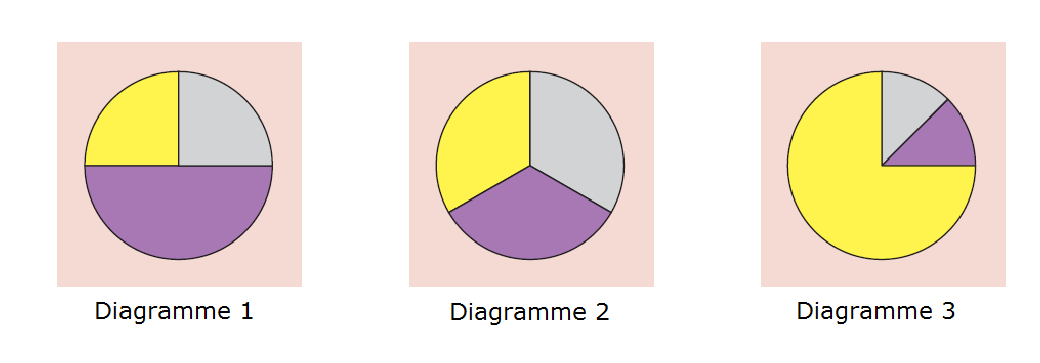
\includegraphics[scale=0.9]{diagramme2.eps} \\
	
	Réponses :\\
	
Diagramme 1 : . . . . . . . .\\

Diagramme 2 : . . . . . . . .\\
	
	Diagramme 3 : . . . . . . . .\\
		



\exo \\ Le diagramme ci-dessous donne la répartition en pourcentage d'adhérent d'un club de tennis de table.\\

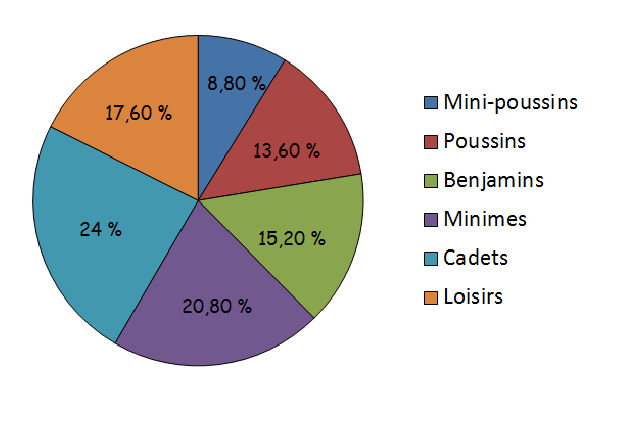
\includegraphics[scale=0.9]{diagramme3.eps} \\
	
	
	\initqa \qa Quel est le pourcentage de Benjamins ? . . . . . . . \\
	
\qa Quel est le pourcentage de Mini-poussins ? . . . . . . . \\

\qa Ce graphique permet-il de connaître le nombre de poussins dans le club ? . . . . . . . \\



\exo \\ Le club météo de la ville de Savray propose ce 	diagramme représentant les précipitations en mai 2017.\\

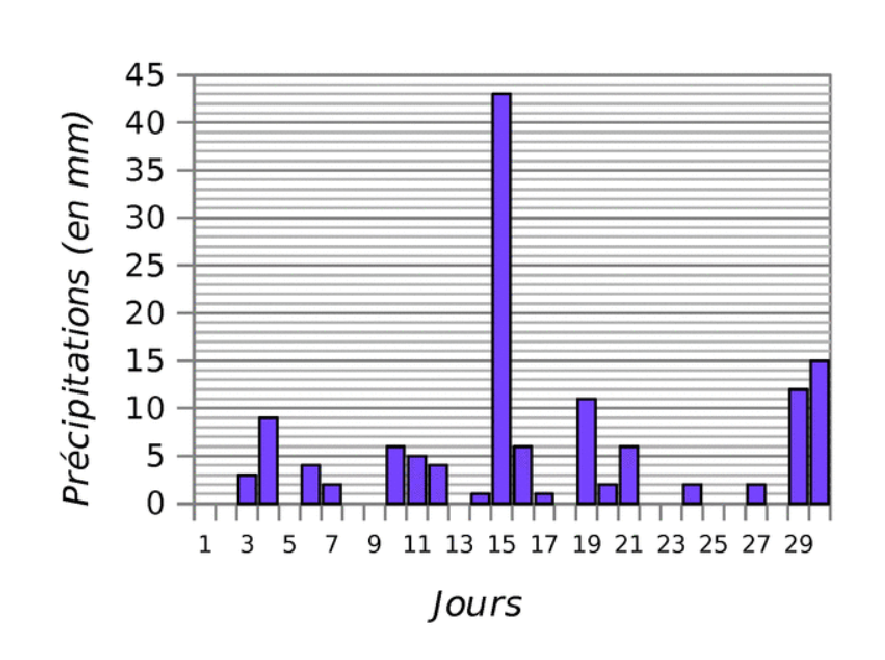
\includegraphics[scale=0.9]{diagramme8.eps} \\

\initqa \qa Quelle quantité d'eau en millimètres est tombée le 21 mai ? . . . . . . . .\\

\qa Quels sont les jours du mois de mai où il n'a pas plut ?\\
\reponse[1]\\





\vspace*{1cm}

$\rightarrow$ \textbf{Exploiter un tableau}\\

\vspace*{0.5cm}





\exo \\ Voici les résultats du contrôle sur 20 de sciences de la classe de 6ème A, aucun absent à ce contrôle.\\

\begin{tabular}{|c|c|c|c|c|c|c|c|}
\hline 
\textbf{Notes} & 7 & 9  & 10 & 12 & 14 & 17 & 19 \\ 
\hline 
\textbf{Nombre d'élèves ayant obtenu cette note}  & 2 & 1 & 4 & 9 & 3 & 6 & 2 \\ 
\hline 
\end{tabular} \\

Qui a raison ?\\

Matéo : "A ce contrôle, 7 élèves ont eu 2."\\

Lucie : "A ce contrôle, seulement 2 élèves ont eu 7."\\


A-ton avis, qui de Matéo ou de Lucie a raison ? . . . . . . . . \\




\exo \\ Voici les résultats du contrôle sur 20 de sciences de la classe de 6ème A, aucun absent à ce contrôle.\\

\begin{tabular}{|c|c|c|c|c|c|c|c|}
\hline 
\textbf{Notes} & 7 & 9  & 10 & 12 & 14 & 17 & 19 \\ 
\hline 
\textbf{Nombre d'élèves ayant obtenu cette note}  & 2 & 1 & 4 & 9 & 3 & 6 & 2 \\ 
\hline 
\end{tabular} \\

\initqa \qa Combien d'élèves ont eu 10 à ce contrôle ? . . . . .\\

\qa Combien d'élèves ont eu 19 à ce contrôle ? . . . . .\\



\exo \\ Voici les résultats du contrôle sur 20 de sciences de la classe de 6ème A, aucun absent à ce contrôle.\\

\begin{tabular}{|c|c|c|c|c|c|c|c|}
\hline 
\textbf{Notes} & 7 & 9  & 10 & 12 & 14 & 17 & 19 \\ 
\hline 
\textbf{Nombre d'élèves ayant obtenu cette note}  & 2 & 1 & 4 & 9 & 3 & 6 & 2 \\ 
\hline 
\end{tabular} \\

Combien d'élèves y a-t-il dans cette classe ? . . . . . . . . . \\







\vspace*{0.5cm}

\begin{center}
{\Large \textbf{Niveau 2 :}}
\end{center}

\vspace*{1cm}

$\rightarrow$ \textbf{Exploiter un diagramme}\\

\vspace*{0.5cm}



\exo \\ Le diagramme ci-dessous donne la répartition selon l'âge dans un groupe d'élèves :\\

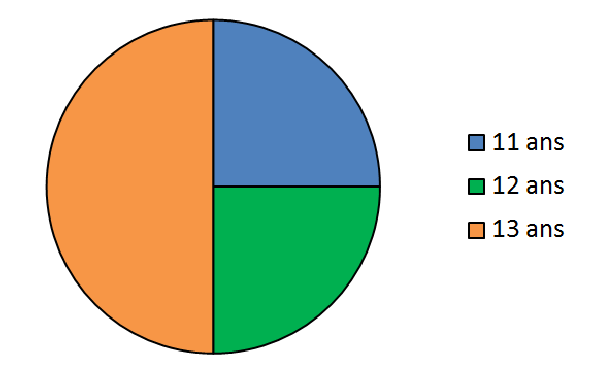
\includegraphics[scale=0.9]{diagramme1.eps} \\

Dans ce groupe, il y a 14 élèves qui ont 11 ans.\\

\initqa \qa Combien d'élèves de ce groupe ont 12 ans ? . . . . . \\

\qa Combien y a-t-il d'élèves dans ce groupe ? . . . . . \\



\exo \\ On a demandé aux élèves d'une classe de 6èmes le nombre de frères puis le nombre de sœurs qu'ils avaient. Voici les résultats.\\


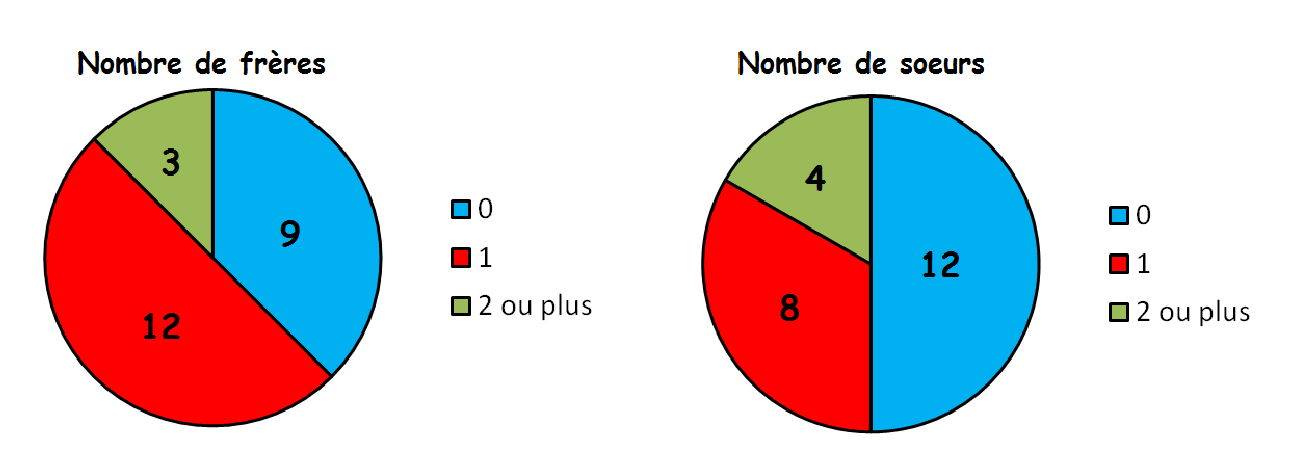
\includegraphics[scale=0.9]{diagramme4.eps} \\


\initqa \qa Combien d'élèves n'ont ni frère ni soeur ? . . . . . . \\




\qa Combien d'élèves ont un frère ? . . . . . . \\



\exo \\ Le graphique ci-dessous représente la répartition des médailles d'or gagnées au Jeux Paralympiques de 2012 pour ces neufs pays.\\


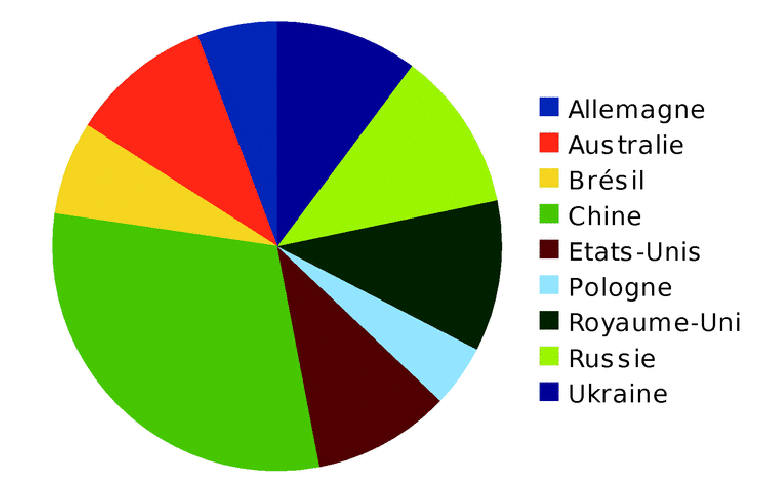
\includegraphics[scale=0.9]{diagramme6.eps} \\

\initqa \qa Quel pays a gagné  le plus de médaille d'or ? . . . . . . . . .\\

\qa Parmi ces neufs pays, quels sont ceux qui ont gagné  moins de médailles d'or  que le Brésil ?\\
\reponse[2]\\

\qa Compléter la phrase suivante :\\
" La Chine a gagné . . . . . fois plus de médailles que les États-Unis.\\

	
\exo \\ Le graphique représente les températures relevées toutes les heures, pendant une journée par une station météo.\\

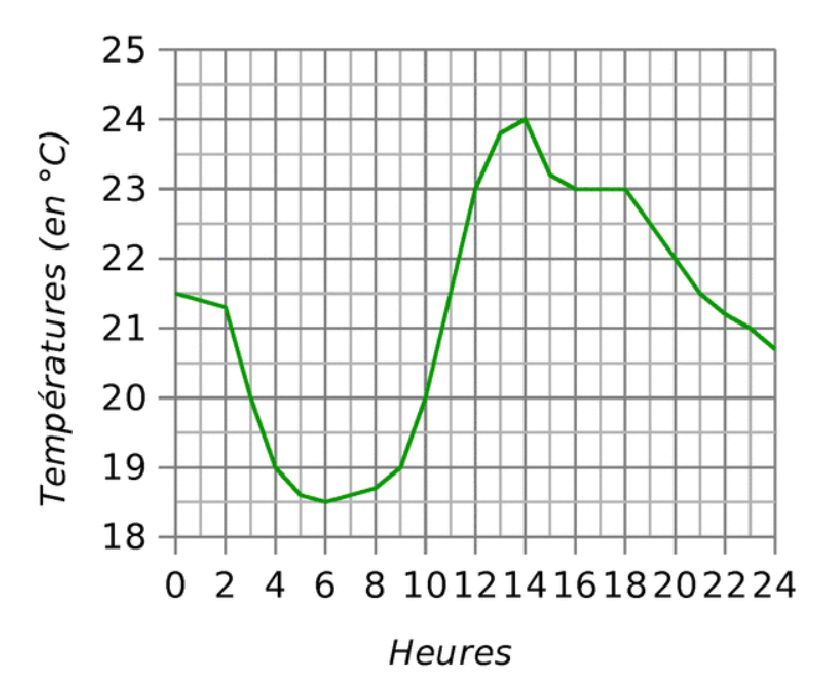
\includegraphics[scale=0.9]{diagramme9.eps} \\

\initqa \qa  Quelle était la température à 4h ? et à 19 h ce jour-là? . . . . . . . .\\

\qa A quelles heures a-t-il fait 20\degre C ? . . . . . . . . . . . .\\


\exo \\ Le graphique représente les températures relevées toutes les heures, pendant une journée par une station météo.\\

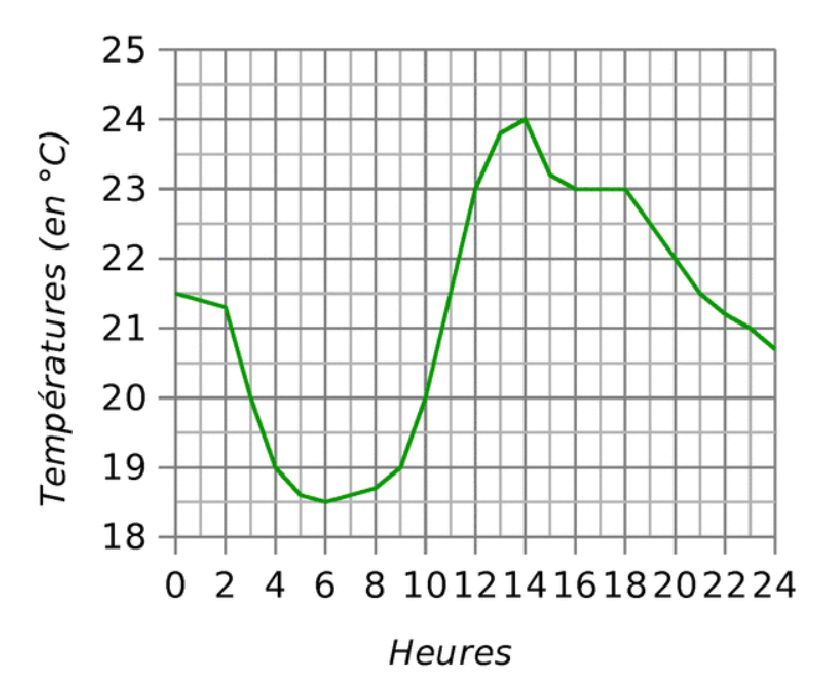
\includegraphics[scale=0.9]{diagramme9.eps} \\

\initqa \qa  Quelle est la température relevé la plus importante et à quelle heure de la journée ? . . . . . . . .\\

\qa \qa  Quelle est la température relevé la plus faible et à quelle heure de la journée ? . . . . . . . .\\

\vspace*{1cm}

$\rightarrow$ \textbf{Exploiter un tableau}\\

\vspace*{0.5cm}






\exo \\ Dans une boîte de jeu, il y a des personnages bleus, des personnes vertes et des personnages rouges. Ils représentent soit des sorciers, soit des fées.\\
Le tableau ci-dessous représente la répartition des personnages en fonction de sa couleur et de sa personnalité.\\


\begin{tabular}{|c|c|c|c|}
\hline 
 & \textbf{Sorciers} & \textbf{Fées} & Total \\ 
\hline 
\textbf{Bleu} & 5 & 3 & 8 \\ 
\hline 
\textbf{Rouge}  & 1 & 2 & 3 \\ 
\hline 
\textbf{Vert} & 7 & 9 & 16 \\ 
\hline 
Total & 13 & 14 & 27 \\ 
\hline 
\end{tabular} \\



 A l'aide du tableau, répondre aux questions suivantes :\\



\initqa \qa Combien de personnages en tout y a-t-il dans la boîte ? . . . . . \\

\qa Combien de personnages verts y a-t-il dans la boîte ? . . . . . \\


\qa Combien de fées y a-t-il dans la boîte ? . . . . . \\




\exo \\ Le tableau ci-dessous donne la répartition des élèves de cinquièmes d'un collège en fonction de leur régime : interne, demi-pensionnaire ou externe.\\

\begin{tabular}{|c|c|c|c|c|}
\hline 
 & Internes & Demi-pensionnaires & Externes & Total \\ 
\hline 
Filles & 5 & 35 & 20 & 60  \\ 
\hline 
Garçon & 10 & 15 & 40	 & 65  \\ 
\hline 
Total & 15 & 50 & 60 & 125  \\ 
\hline 
\end{tabular} \\

Vrai ou Faux.\\


\initqa \qa Il y a 5 filles externes. \textbf{Vrai ou Faux.}\\

\qa Il y a 40 garçons externes. \textbf{Vrai ou Faux.}\\

\qa Il y a en tout 35 demi-pensionnaires. \textbf{Vrai ou Faux.}\\



\exo \\ Voici les résultats du contrôle sur 20 de sciences de la classe de 6ème A, aucun absent à ce contrôle.\\

\begin{tabular}{|c|c|c|c|c|c|c|c|}
\hline 
\textbf{Notes} & 7 & 9  & 10 & 12 & 14 & 17 & 19 \\ 
\hline 
\textbf{Nombre d'élèves ayant obtenu cette note}  & 2 & 1 & 4 & 9 & 3 & 6 & 2 \\ 
\hline 
\end{tabular} \\

\initqa \qa Combien d'élèves ont eu plus de 10 à ce contrôle ? . . . . .\\

\qa Combien d'élèves ont eu moins de 14 à ce contrôle ? . . . . .\\

\qa Combien d'élèves ont eu au moins 12 à ce contrôle ? . . . . .\\


\vspace*{0.5cm}







\begin{center}
{\Large \textbf{Niveau 3 :}}
\end{center}

\vspace*{1cm}

$\rightarrow$ \textbf{Exploiter un diagramme}\\

\vspace*{0.5cm}



\exo \\ On a demandé aux élèves d'une classe de 6èmes le nombre de frères puis le nombre de sœurs qu'ils avaient. Voici les résultats.\\


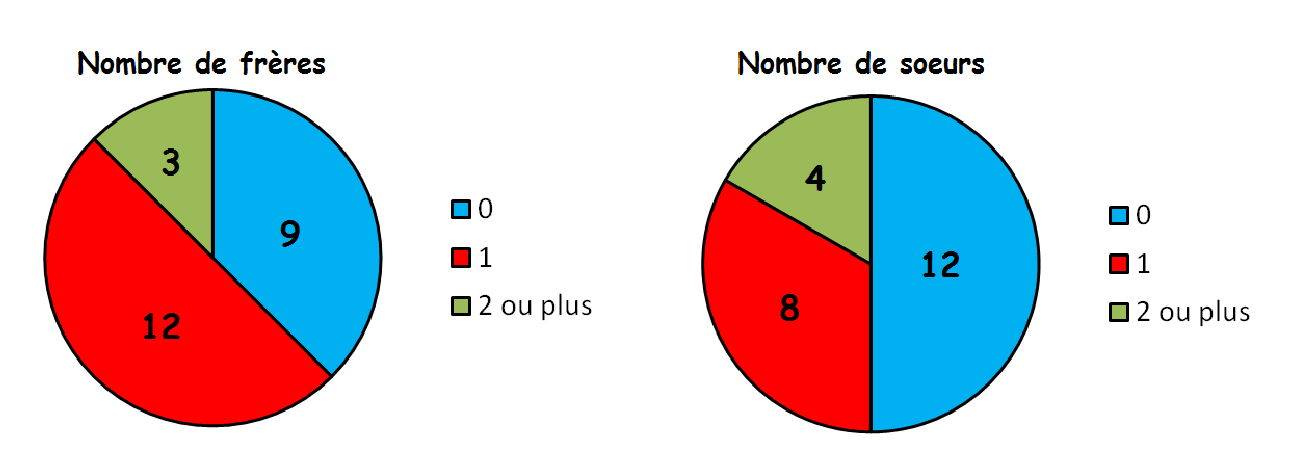
\includegraphics[scale=0.9]{diagramme4.eps} \\


\initqa \qa Combien d'élèves ont au moins un frère et une soeur ? . . . . . . \\




\qa Combien d'élèves ont deux soeurs ou plus ? . . . . . . \\


\exo \\ Les diagrammes suivants représentent la répartition en pourcentage des indices de masse corporelle des français  en 1995 et en 2009.\\

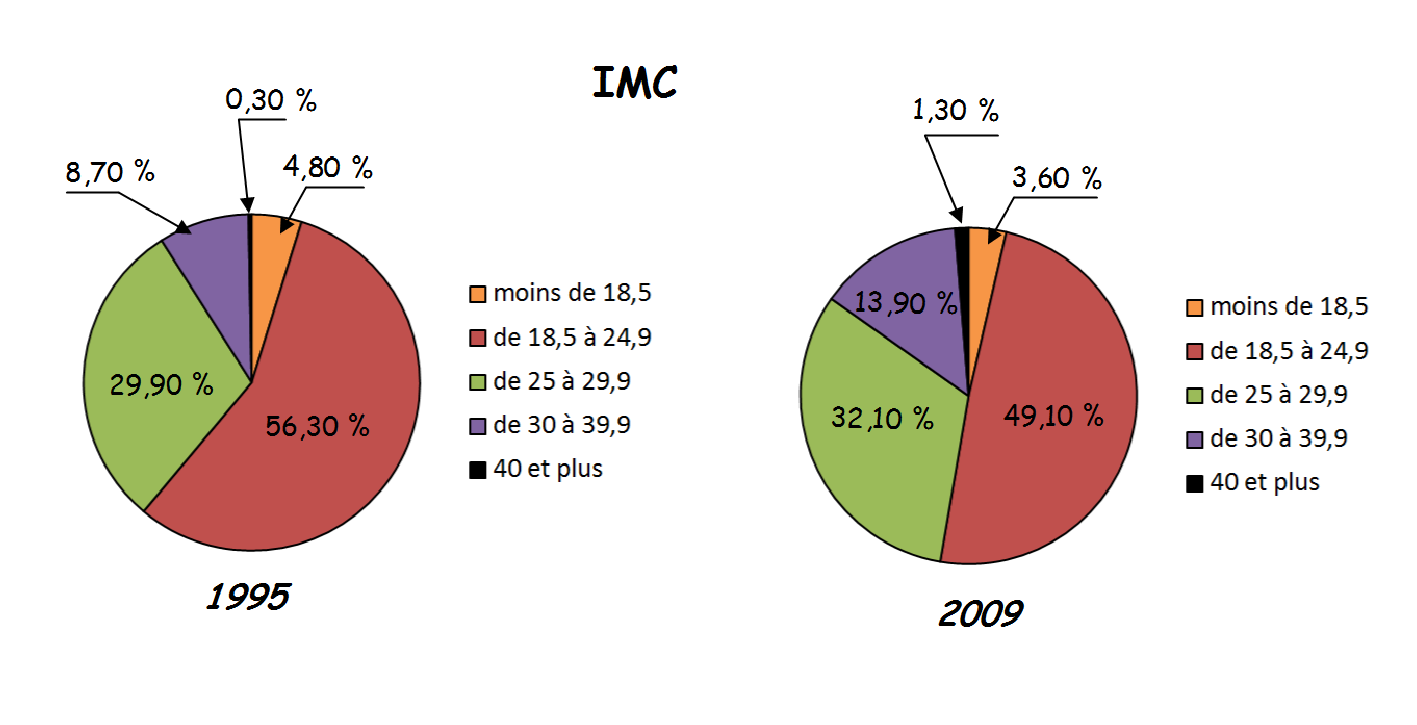
\includegraphics[scale=0.8]{diagramme7.eps} \\

\begin{tabular}{|c|c|}
\hline 
\textbf{IMC (Indice de Masse Corporelle)} & \textbf{Classification} \\ 
\hline 
moins de 18,5 & Maigreur  \\ 
\hline 
de 18,5 à 24,9 & Corpulence normale \\ 
\hline 
de 25 à 29,9 & Surpoids \\ 
\hline 
de 30 à 39,9 & Obésité modérée \\ 
\hline 
40 et plus & Obésité morbide \\ 
\hline 
\end{tabular} \\

\initqa \qa Quel est le pourcentage des individus ayant un IMC inférieur à 18,5 en 2009 ? . . . . . . . \\

\qa Quel est le pourcentage des individus étant en surpoids en 1995 ? . . . . . . . . . .\\


\qa Le pourcentage d'individus de corpulence normale a-t-il augmenté ou diminué de 1995 à 2009 ? . . . . . . . . . .\\


\exo \\ Le club météo de la ville de Savray propose ce 	diagramme représentant les précipitations en mai 2017.\\

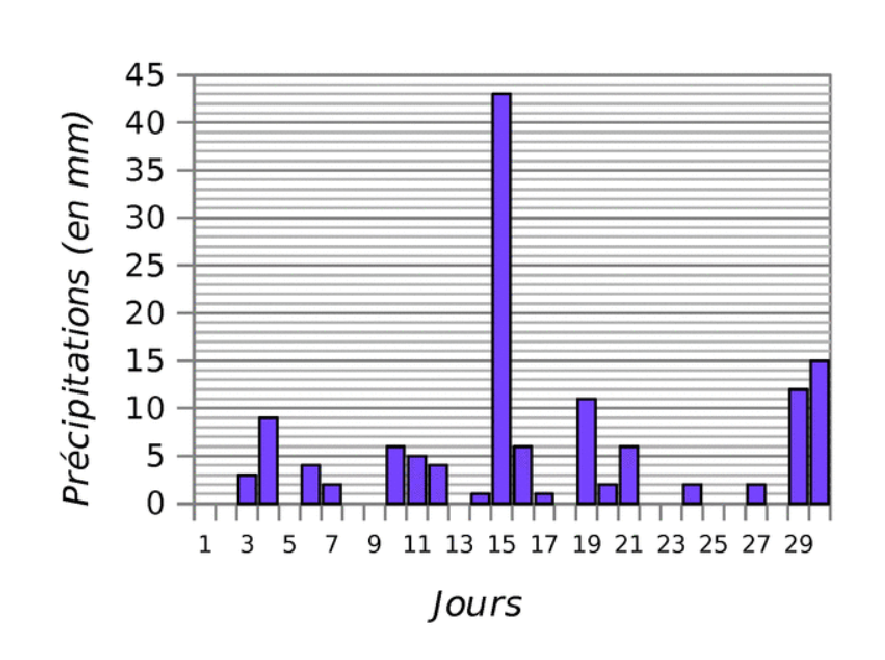
\includegraphics[scale=0.9]{diagramme8.eps} \\

\initqa  \qa Combien de jours est-il tombé plus de 8 mm  de pluie ? . . . . . . . \\

\qa Quelle quantité d'eau en millimètres est-il tombée entre le 1 et le 11 mai ? . . . . . . . . . . . . . . . . .\\


\exo \\ Ce graphique représente les naissances en France entre 2003 et 2011.\\


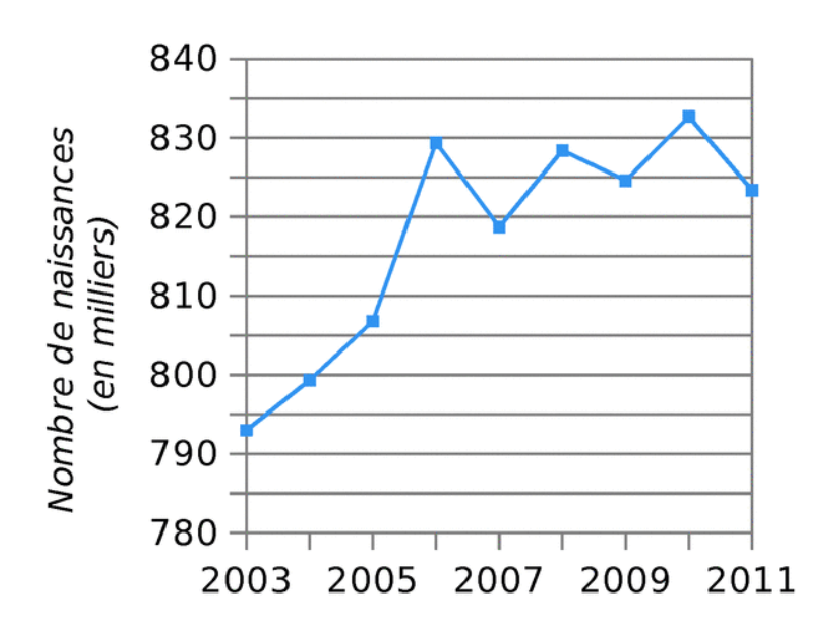
\includegraphics[scale=0.9]{diagramme10.eps} \\


\initqa \qa Entre 2003 et 2011, en quelle année y a-t-il eu le plus de naissance ? . . . . . . . . . .\\

\qa Que peut-on dire des naissances entre 2003 et 2006 ? . . . . . . .\\

\qa En quelle année y a-t-il eu plus de 815 000 naissances en France ? . . . . . . . . . . .\\




\vspace*{1cm}

$\rightarrow$ \textbf{Exploiter un tableau}\\

\vspace*{0.5cm}


\exo \\ Dans une boîte de jeu, il y a des personnages bleus, des personnes vertes et des personnages rouges. Ils représentent soit des sorciers, soit des fées.\\
Le tableau ci-dessous représente la répartition des personnages en fonction de sa couleur et de sa personnalité.\\


\begin{tabular}{|c|c|c|c|}
\hline 
 & \textbf{Sorciers} & \textbf{Fées} & Total \\ 
\hline 
\textbf{Bleu} & 5 & 3 & 8 \\ 
\hline 
\textbf{Rouge}  & 1 & 2 & 3 \\ 
\hline 
\textbf{Vert} & 7 & 9 & 16 \\ 
\hline 
Total & 13 & 14 & 27 \\ 
\hline 
\end{tabular} \\



 A l'aide du tableau, répondre aux questions suivantes :\\



\initqa \qa Combien de sorciers en tout y a-t-il dans la boîte ? . . . . . \\

\qa Combien de fées vertes y a-t-il dans la boîte ? . . . . . \\


\qa Si on retire les personnages verts de la boîte, combien de personnages  reste-t-il ? . . . . . \\



\exo \\ Le tableau ci-dessous donne la répartition des élèves de cinquièmes d'un collège en fonction de leur régime : interne, demi-pensionnaire ou externe.\\

Des cases du tableau ont été effacées, saurez-vous retrouver ce qu'il y avait d'écrit.\\

\begin{tabular}{|c|c|c|c|c|}
\hline 
 & Internes & Demi-pensionnaires & Externes & Total \\ 
\hline 
Filles & 7 & 34 & 19 & . . . .  \\ 
\hline 
Garçon & 8 & 16 & 41	 & . . . .  \\ 
\hline 
Total & . . . . & . . . . & . . . . & . . . .  \\ 
\hline 
\end{tabular} \\




\exo \\ Le tableau ci-dessous donne la répartition des élèves de cinquièmes d'un collège en fonction de leur régime : interne, demi-pensionnaire ou externe.\\

\begin{tabular}{|c|c|c|c|c|}
\hline 
 & Internes & Demi-pensionnaires & Externes & Total \\ 
\hline 
Filles & 5 & 35 & 20 & 60  \\ 
\hline 
Garçon & 10 & 15 & 40	 & 65  \\ 
\hline 
Total & 15 & 50 & 60 & 125  \\ 
\hline 
\end{tabular} \\

Vrai ou Faux.\\


\initqa \qa Dans ce collège, il y a plus de garçons que de filles. \textbf{Vrai ou Faux.}\\

\qa La proportion d'internes parmi tous les élèves est $\dfrac{5}{125}$. \textbf{Vrai ou Faux.}\\

\qa Il y a la même proportion de filles parmi les internes que parmi les externes. \textbf{Vrai ou Faux.}\\







\begin{center}
{\Large \textbf{Niveau 4:}}
\end{center}

\vspace*{1cm}

$\rightarrow$ \textbf{Exploiter un diagramme}\\

\vspace*{0.5cm}





\exo \\ On a demandé aux élèves d'une classe de 6èmes le nombre de frères puis le nombre de sœurs qu'ils avaient. Voici les résultats.\\


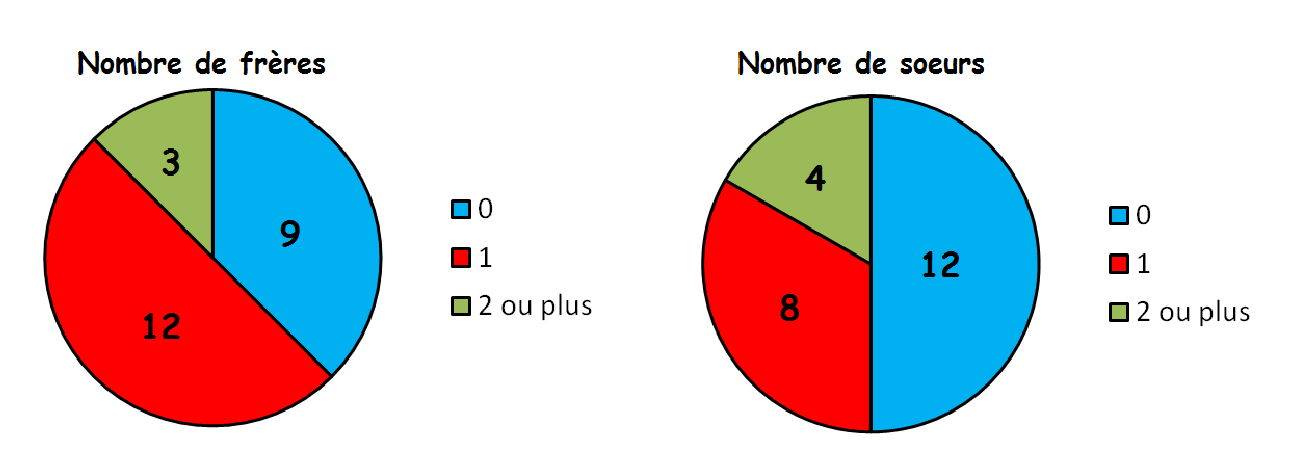
\includegraphics[scale=0.9]{diagramme4.eps} \\


\initqa \qa Combien d'élèves n'ont que des frères ? . . . . . . \\




\qa Combien d'élèves n'ont pas de soeur ? . . . . . . \\


\exo \\ Dans un collège, on a demandé aux 200 élèves de cinquièmes s'ils possédaient un animal de compagnie et  si oui, lequel? Voici les résultats de l'enquête.\\

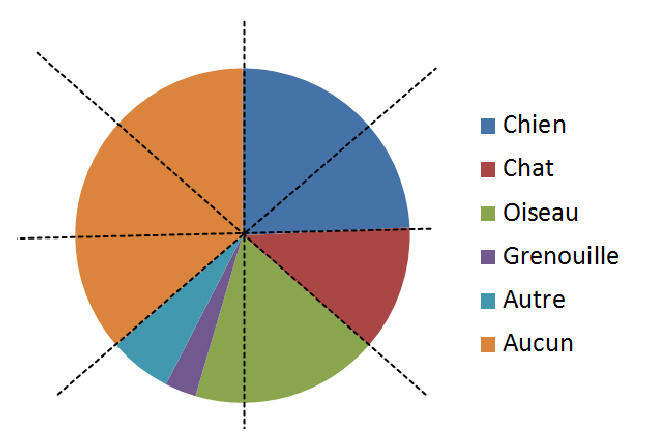
\includegraphics[scale=0.9]{diagramme5b.eps} \\

Répondre par vrai ou par faux.\\



\initqa \qa Les élèves  qui ont une grenouille  sont plus nombreux que ceux qui ont un chat. \textbf{Vrai ou Faux.}\\

\qa Un quart des élèves ont un oiseau. \textbf{Vrai ou Faux.}\\

\qa Moins des trois quarts des élèves ont un animal de compagnie. \textbf{Vrai ou Faux.}\\

\qa Les élèves  qui ont un chat sont moitié moins nombreux que ceux qui ont un chien. \textbf{Vrai ou Faux.}\\


	
\vspace*{1cm}

$\rightarrow$ \textbf{Exploiter un tableau}\\

\vspace*{0.5cm}




\exo \\ Dans une boîte de jeu, il y a des personnages bleus, des personnes vertes et des personnages rouges. Ils représentent soit des sorciers, soit des fées.\\
On sait qu'il y a 8 personnages bleus, 13 sorciers, 5 sorciers bleus, 16 personnages verts, 9 fées verts et 27 personnages en tout dans la boîte.\\

Compléter le tableau récapitulatif ci-dessous.\\


\begin{tabular}{|c|c|c|c|}
\hline 
 & \textbf{Sorciers} & \textbf{Fées} & Total \\ 
\hline 
\textbf{Bleu} & 5 & . . . & 8 \\ 
\hline 
\textbf{Rouge}  & . . . & . . . & . . . \\ 
\hline 
\textbf{Vert} & . . . & . . . & 16 \\ 
\hline 
Total & 13 & . . . & 27 \\ 
\hline 
\end{tabular} \\





\exo \\ Les adhérents d'un club de la ville de Montrouge se répartissent selon le tableau ci-dessous.\\

\begin{tabular}{|c|c|c|}
\hline 
 & Hommes & Femmes \\ 
\hline 
Pratiquent un sport & 57 & 26 \\ 
\hline 
Ne pratiquent pas de sport & 21 & 32 \\ 
\hline 
\end{tabular} \\

\initqa \qa Combien y a-t-il d'adhérents dans ce club? . . . . . . \\

\qa Combien y a-t-il de femmes dans ce club? . . . . . . \\

\qa Combien y a-t-il d'hommes dans ce club? . . . . . . \\ 





\exo \\ Dans un magasin, on fait l'inventaire des tee-shirts. Il y a 30 tee-shirts à manches courtes ou à manche longue, de couleur bleue, rouge ou blanc.\\

On sait qu'il y a : \\

- 12 tee-shirt bleus ; \\

- 10 tee-shirt à manches courtes ; \\

- 5 tee-shirt blancs à manches longues ; \\

- 2 tee-shirt bleus à manches courtes ; \\

- 8 tee-shirts blancs.\\

\begin{tabular}{|c|c|c|c|}
\hline 
 & Manches courtes & Manches longues & Total \\ 
\hline 
Bleu & . . .  & . . . & . . . \\ 
\hline 
Rouge & . . .  & . . . & . . . \\  
\hline 
Blanc & . . .  & . . . & . . . \\ 
\hline 
Total & . . .  & . . . & . . . \\ 
\hline 
\end{tabular} 












\begin{center}
{\Large \textbf{Niveau 5 :}}
\end{center}

\vspace*{1cm}

$\rightarrow$ \textbf{Exploiter un diagramme}\\

\vspace*{0.5cm}


\exo \\ Dans un collège, on a demandé aux 200 élèves de cinquièmes s'ils possédaient un animal de compagnie et  si oui, lequel? Voici les résultats de l'enquête.\\

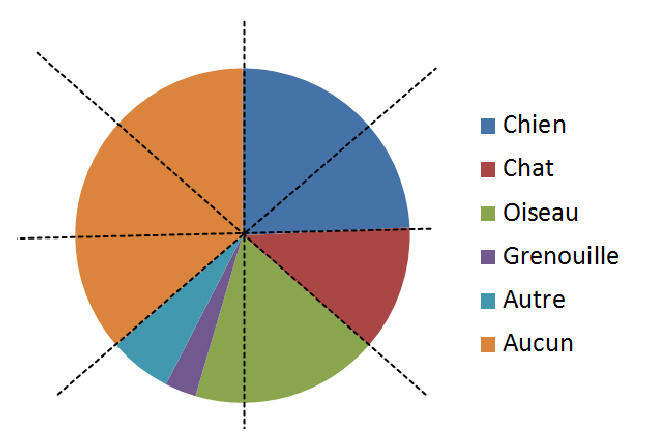
\includegraphics[scale=0.9]{diagramme5b.eps} \\

\initqa \qa Combien d'élèves possèdent un chien ? . . . . .\\

\qa Combien d'élèves possèdent un chat ? . . . . .\\





\exo \\ Les diagrammes suivants représentent la répartition en pourcentage des indices de masse corporelle des français  en 1995 et en 2009.\\

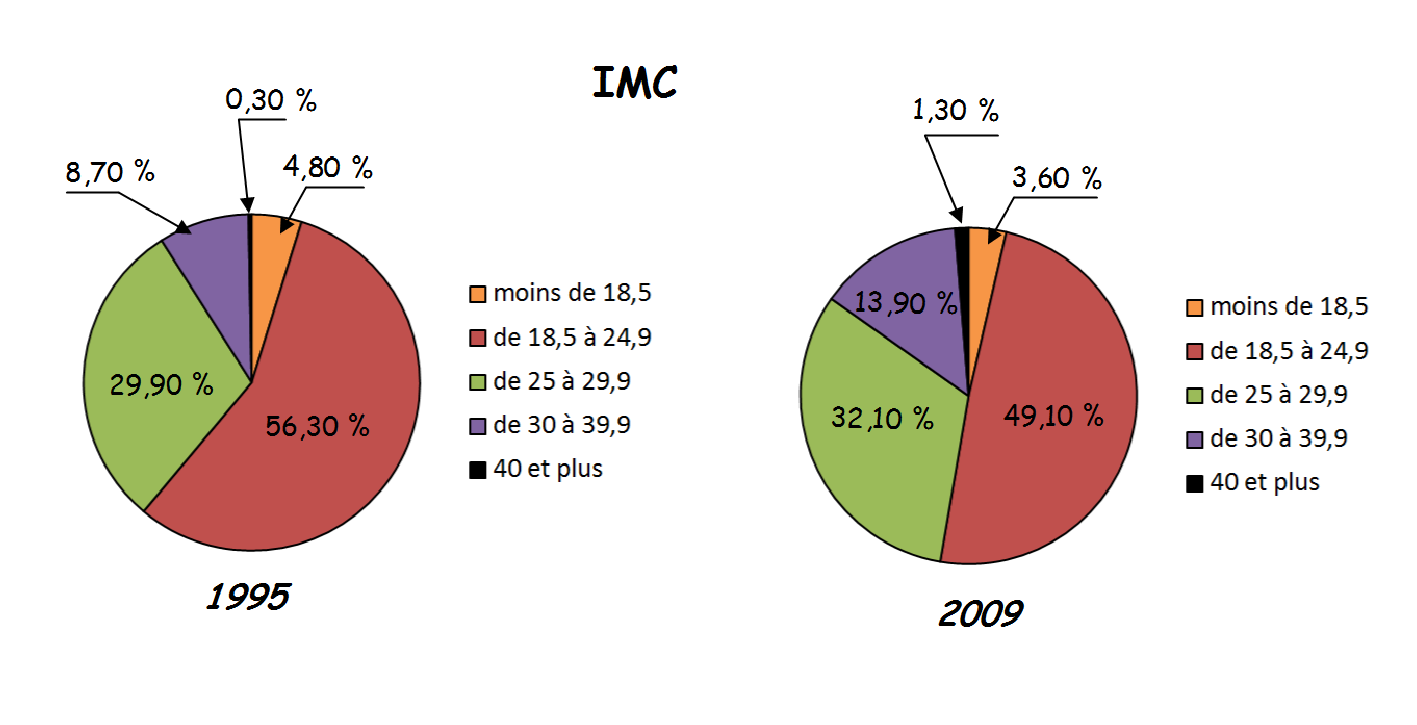
\includegraphics[scale=0.8]{diagramme7.eps} \\

\begin{tabular}{|c|c|}
\hline 
\textbf{IMC (Indice de Masse Corporelle)} & \textbf{Classification} \\ 
\hline 
moins de 18,5 & Maigreur  \\ 
\hline 
de 18,5 à 24,9 & Corpulence normale \\ 
\hline 
de 25 à 29,9 & Surpoids \\ 
\hline 
de 30 à 39,9 & Obésité modérée \\ 
\hline 
40 et plus & Obésité morbide \\ 
\hline 
\end{tabular} \\

\initqa \qa Quel est le pourcentage des individus ayant un IMC supérieur ou égal à 30 en 1995 ? . . . . . . . \\

\qa Un individu est obèse lorsque son IMC est égal ou supérieur à 30. Le pourcentage de personnes obèses est-elle plus importante en 1995 ou en 2009 ? . . . . . . . . .\\

\qa  La moitié des individus sont de corpulence normale en 1995. \textbf{Vrai ou faux ?}  . . . . . . . . . .\\


\qa La moitié des individus sont de corpulence normale en 2009. \textbf{Vrai ou faux ?} . . . . . . . . . .\\


\exo \\ Le graphique suivant représente le poids (en kg) de Jules en fonction de son  âge. \\
Les courbes en \textcolor{red}{rouge} représentent les poids minimum et maximum conseillés.\\


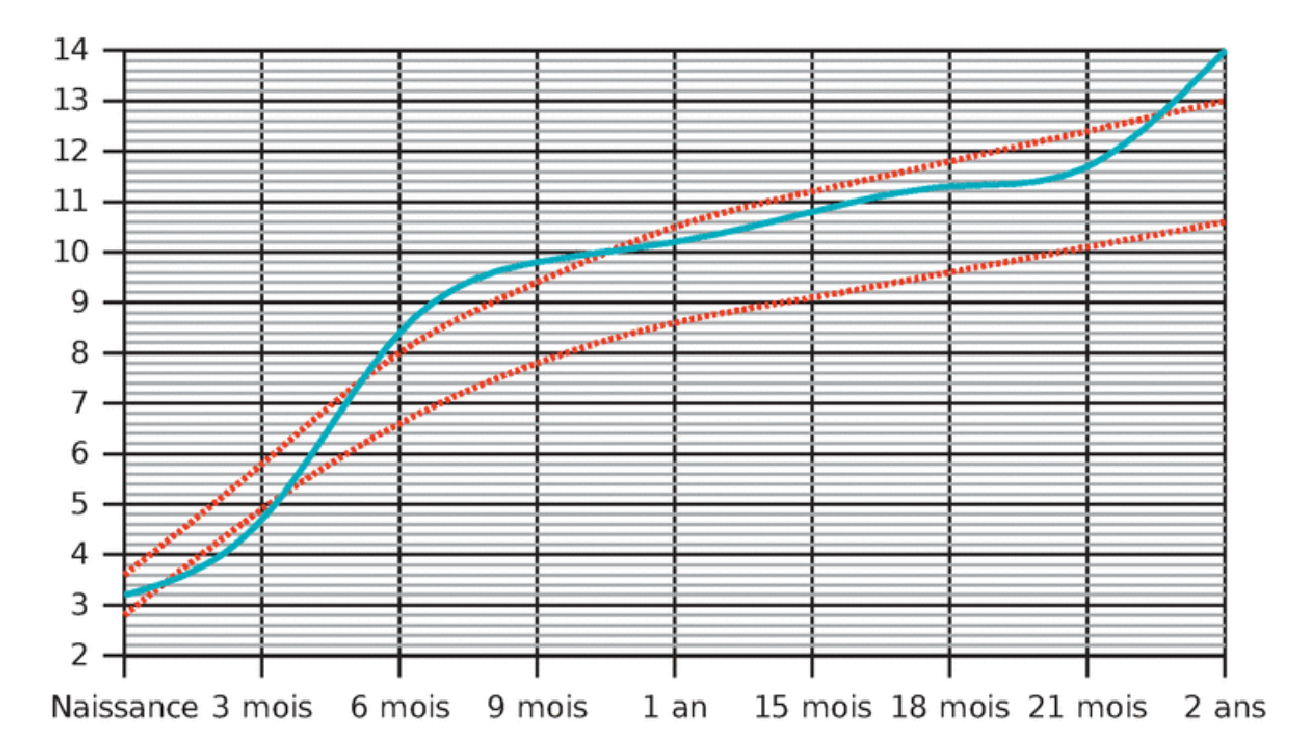
\includegraphics[scale=0.8]{diagramme11.eps} \\


\initqa


\qa A quels âges, Jérôme est-il au dessus du poids conseillé ? . . . . . . . . .\\

\qa De combien de kilogrammes son poids a-t-il augmenté entre ses 1 an et ses 2 ans ? . . . . . . . . . . \\ 





\vspace*{1cm}

$\rightarrow$ \textbf{Exploiter un tableau}\\

\vspace*{0.5cm}





\exo \\ Les adhérents d'un club de la ville de Montrouge se répartissent selon le tableau ci-dessous.\\

\begin{tabular}{|c|c|c|}
\hline 
 & Hommes & Femmes \\ 
\hline 
Pratiquent un sport & 57 & 26 \\ 
\hline 
Ne pratiquent pas de sport & 21 & 32 \\ 
\hline 
\end{tabular} \\

Cliquer sur la bonne réponse.\\




\begin{tabular}{|c|c|c|c|}
\hline 
Parmi les hommes la proportion de ceux qui pratiquent un sport est de ... & $\dfrac{57}{21}$ & $\dfrac{57}{78}$ & $\dfrac{57}{136}$ \\ 
\hline 
Dans ce club, la proportion des femmes est de ... & $\dfrac{26}{57}$ & $\dfrac{32}{21}$ & $\dfrac{58}{136}$ \\ 
\hline 
Dans ce club, la proportion des adhérents pratiquants le sport est de ... & $\dfrac{57}{78}$ & $\dfrac{83}{136}$ & $\dfrac{26}{32}$ \\  
\hline 
\end{tabular} 



\exo \\ Dans le village de Vallon,  Yann, Céline et Mélanie ont rassemblé leurs animaux en un troupeau pour effectuer la transhumance ensemble.\\
Le tableau ci-dessous donne la répartition des brebis, béliers et moutons pour chacun d'eux.\\

Le tableau n'est malheureusement pas complet, à toi de le compléter.\\

\begin{tabular}{|c|c|c|c|c|}
\hline 
 & \textbf{Brebis} & \textbf{Bélier} & \textbf{Mouton} & \textbf{Total} \\ 
\hline 
\textbf{Yann} & 160 & 30 & . . . . & 800 \\ 
\hline 
\textbf{Céline} & . . . . & 20 & 700 & . . . . \\ 
\hline 
\textbf{Mélanie} & . . . . & . . . . & . . . . & 700 \\ 
\hline 
\textbf{Total} & 540 & . . . . & 1900 & 2500 \\ 
\hline 
\end{tabular} 


\vspace*{1cm}




\exo \\ Dans la boîte à bonbons de Luc, il y a deux sortes de bonbons : des crocodiles et des oursons.\\
Il y en a des rouges, des verts et des jaunes.\\

On sait que : \\

- $\dfrac{2}{3}$ des bonbons sont des crocodiles.\\

- $\dfrac{1}{5}$ des oursons sont rouges.\\

- Il y a 50 bonbons jaunes.\\

- Il y a deux fois plus de crocodiles rouges que d'oursons rouges.\\

- Il y a trois fois plus d'oursons jaunes que d'oursons rouges.\\

- Il y a en tout 150 bonbons.\\


\begin{tabular}{|c|c|c|c|c|}
\hline 
 & \textbf{Rouge} & \textbf{Vert} & \textbf{Jaune} & \textbf{Total} \\ 
\hline 
\textbf{Les crocodiles} & . . . . & . . . . & . . . . & . . . . \\ 
\hline 
\textbf{Les oursons} & . . . . & . . . . & . . . . & . . . . \\ 
\hline 
\textbf{Total} & . . . . & . . . . & . . . . & 150 \\ 
\hline 
\end{tabular} 







\end{document}
